\documentclass[tikz]{standalone}
\usepackage{bm}
\newcommand{\vect}{\bm}
\newcommand{\del}{\boldsymbol{\nabla}}

\begin{document}
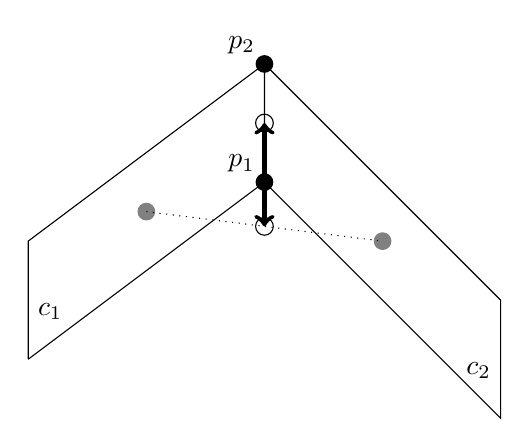
\begin{tikzpicture}[
  scale=0.75,
  cpnt/.style={fill=gray},
  vertex/.style={fill=black},
  arr/.style={ultra thick, <->},
  mag/.style={dashed, thick, <->}
]
\draw (0,0) -- (4,3) -- (4,5) -- (0,2) -- (0,0);
\draw (4,3) -- (8,-1) -- (8,1) -- (4,5);
\node [above right] at (0,0.5) {$c_1$};
\node [above left] at (8,-0.5) {$c_2$};

\path [vertex] (4,3) circle [radius=0.15] node [above left] {$p_1$};
\path [vertex] (4,5) circle [radius=0.15] node [above left] {$p_2$};

\path [cpnt] (2,2.5) circle [radius=0.15];
\path [cpnt] (6,2) circle [radius=0.15];

\draw (4,4) circle [radius=0.15];
\draw (4,2.25) circle [radius=0.15];
\draw [dotted] (2,2.5) -- (6,2);
\draw [arr] (4,4) -- (4,2.25);
\end{tikzpicture}
\end{document}
